\chapter{conclusion}\label{ch:conclusion}

\section{contributions}
This thesis presented a framework to reconstruct Alethe-format SMT proofs into the $\lp$-calculus modulo rewriting.
The contributions of this work are both conceptual and practical.
On the conceptual side, we designed a systematic encoding of SMT logics, including first-order reasoning and linear arithmetic, into a dependently typed setting that includes rewriting logic.
This encoding allows us to faithfully represent Alethe inference rules, and to verify them inside the trusted kernel of Lambdapi.
On the practical side, we developed a modular extension of Carcara \cite{carcara} to translate Alethe proof into Lambdapi. This extension leverage elaboration pipeline of Carcara and RARE \cite{rare} of cvc5 \cite{cvc5}.
Following the approach of \emph{proof logging} \cite{proof-logging}, this methodology yields independently checkable proof certificates, ensuring that solver outputs can be validated without relying on the internal correctness of the solver itself.

Our approach extends the usability of Alethe by providing a certified reconstruction pipeline that increase trust of SMT proofs.
Moreover, we can benefit of the Lambdapi features of import and exporting proof \cite{blanqui:hal-04613926} to share SMT proof in order to increase portability, and interoperability across different proof assistants.


\paragraph{Encoding SMT-LIB in Lambdapi}
A first contribution is the encoding of the syntax and semantics of SMT-LIB into Lambdapi.
We defined universes for sorts, terms, and formulas, together with embeddings that map SMT-LIB constructs into Lambdapi constructions.
This encoding supports equality, logical connectives, quantifiers, and arithmetic operators, and it serves as the foundation for the reconstruction of Alethe proofs.
By encoding SMT-LIB's many-sorted first-order logic with dependent types and rewriting in Lambdapi, we enable a faithful and extensible representation of SMT solver proof traces that can interact with other formal libraries.
Besides, this work also significantly extended the current standard library of Lambdapi.

\paragraph{Reconstructing FOL}
We developed a systematic reconstruction of first-order reasoning (logic UF) in Lambdapi.
This includes tautological rules, resolution, quantifier instantiation and skolemization, which were encoded as dedicated lemmas and verified within the kernel.
Special care was taken to handle Alethe’s subproof mechanism and to preserve the structure of natural-deduction style derivations.
This reconstruction demonstrates that a wide range of coarse-grained Alethe rules can be faithfully re-expressed in a fine-grained and certifiable way, thus bridging solver-level reasoning and proof assistant checking.

\paragraph{Reconstruction via reflection}
For proof rules with complex side conditions or computations (e.g., arithmetic simplifications, AC modulo), we encode the side condition as a reflective decision procedure, formally verified in Lambdapi.
The proof rule is then reformulated as a theorem where the side condition appears as an explicit premise.

\paragraph{Reconstructing arithmetic}
The reconstruction framework supports proofs in linear arithmetic, both over integers (LIA) and partly over reals (LA).
Here we relied on proof by reflection, implementing normalization procedures for arithmetic expressions within Lambdapi and proving their correctness once and for all.
This approach allowed us to certify simplification rules such as linear combination, equivalence of normalized forms, and inequality reasoning.
In practice, this makes it possible to validate arithmetic reasoning steps from cvc5, including those elaborated by Carcara’s \texttt{lia\_generic} rule, in an efficient and scalable way.

\paragraph{Reconstructing TLAPS proofs}
A distinctive application of our framework is the reconstruction of proofs produced by the \tlaplus Proof System (\tlaps).
The proof assistant \tlaps uses external SMT solvers such as veriT and cvc5 as backends to discharge proof obligations that arise in the verification of \tlaplus specifications.
By translating these Alethe proofs into Lambdapi, our pipeline provides certified validation of the SMT reasoning steps used inside \tlaps.
This bridges the gap between high-level system proofs in \tlaplus and low-level certified reasoning, and demonstrates that our approach is not limited to isolated SMT benchmarks but also scales to practical verification tasks.

\bigskip

Our empirical evaluation demonstrates that our framework is capable of validating non-trivial SMT traces efficiently, including proofs produced by cvc5 from \tlaps and SMT-LIB benchmarks.

\section{Future Perspective}

These findings lay the groundwork for future investigations into:


\paragraph{Implementing Bitvectors}
A natural extension of this work is the support for the SMT-LIB \textbf{BV} theory.
Although the Alethe format already mentions bitvectors, only three rules are currently supported, and the remainder of the theory is still under specification. 
We are considering to encode bitvectors of width $w$ as elements of the finite type $\kw{Fin}(2^w)$ (\cref{def:fin-def}), i.e.\ natural numbers bounded by $2^w$.
This representation captures the intended semantics of unsigned machine integers and enforces range-safety through dependent typing. 
Arithmetic operators can be defined by lifting operations on $\N$ modulo $2^w$, while bit-level operators such as conjunction, disjunction, or shifts can be defined either via Boolean decomposition of the underlying representation or through modular arithmetic formulations.  
An initial work has been started in this direction for extending the Lambdapi standard library with bitvector.
We chose the $\mathop{Fin}$ representation over other possible encodings due to its relative efficiency.
If, in the future, Lambdapi's kernel adds support for efficient representations of natural numbers e.g.,
via overriding them with arbitrary-precision arithmetic libraries like GMP\footnote{\url{https://gmplib.org/}} bitvectors encoded with $\mathop{Fin}$ would likewise benefit from such optimizations.
We therefore chose to implement $\mathop{Fin}\,n$, as we believe it provides the most suitable and future-proof foundation for representing the $\mathop{BitVec}$ type,
particularly in light of potential enhancements to the kernel.

\begin{definition}[Fin]\label{def:fin-def}
The type $\mathop{Fin} n$ is the type of natural numbers $i$ with the constraint that $i < n$.
It is the canonical type with $n$ elements.
\begin{align*}
& Fin~(n: \N) \coloneq \Sigma~(\lambda\,x, istrue(x < n)) \\
& FinMk~(n: \N) (m: \N) (islt: \prf (m < n)) : Fin~n \\
&\quad\is exist~(\lambda\,x, istrue(x <n))~m~islt\\
&\mathop{val}~[n]: \mathop{Fin} n \ra \N \is \lambda e, e~s\_1 \\
&\mathop{isLt}~[n] (f: \mathop{Fin} n): \prf (f~s_1 < n) \is f~s_2\\
\end{align*}
\end{definition}

\begin{definition}[Bitvector]\label{def:bv-def}
We can define bitvectors as natural numbers bounded by powers of two and modular arithmetic representation.
We first introduce an infix exponentiation function $\_\,\hat{}\,\_$ on $\N$.
Using this, we define the type $BitVec~n$ as the finite type $Fin~(2~\hat~n)$ (written $Fin~2^n$), representing the set of natural numbers strictly less than $2^n$.
\begin{align*}
& \hat{}: \N \ra \N \ra \N \qquad \text{(written infix)}\\
& 0 ~\hat{}~ 1 \re 1 \N\\
& n ~\hat{}~ (m + 1) \re n * (n ~\hat{}~ m)\\[1em]
&BitVec~n \is Fin~(2^n) \\
& mkBv: \Pi(n~m: \N)(p: \prf~(istrue(n < 2^n))): BitVec~n\\
&\quad\is FinMk~(2^n)~m~p
\end{align*}
Each bitvector of size $n$ is thus a natural number modulo $2^n$, capturing the behaviour of (unsigned) integers with $n$ bits.
The function $mkBv$ then takes a size $n: \N$, an element $m$, and a proof $p$ that $m < 2^n$, and returns a bitvector of type $BitVec~n$.
Internally, this is constructed using $FinMk$, the constructor for the finite type $Fin~(2^n)$, ensuring that only values within the correct range can inhabit the bitvector type.
\end{definition}


\paragraph{Eunoia Compatibility} 
Another line of work is to extend our Carcara module to support Alethe proof trace expressed in Eunoia syntax. 
Because the syntaxes of Alethe and Eunoia are closely related, this adaptation appears feasible and would provide a bridge between the two formats, ensuring compatibility with SMT 3 and promoting interoperability across proof exchange ecosystems.


\paragraph{Exporting proof to Rocq}
At present, Lambdapi can only translate its $\lambda$-terms into Coq, which allows a direct re-use of proof objects inside the Rocq ecosystem.
However, this translation only captures the final proof terms and does not reflect the structure of the tactics used in their construction. 
A complementary approach would therefore be to translate Lambdapi tactics into equivalent Rocq tactics or to define new Ltac tactics mirroring their behaviour. 
This would preserve higher-level proof strategies and improve readability and maintainability. 

Another promising direction arises from the recent experimental addition of user-defined rewrite rules in Rocq \cite{rw-rocq}. 
In earlier versions, rewrite rules had to be simulated through \textcolor{lpurple}{\textbf{\kw{Fixpoint}}} definitions, which imposed syntactic guards restricting recursion to structural cases. 
This made it impossible to directly express nonstructural or general recursion, as illustrated by our reflective implementation of merge sort for \texttt{lia\_generic}. 
With Rocq’s new native support for rewriting rules, it becomes feasible to export Lambdapi rewrite rules directly, avoiding the limitations of \textcolor{lpurple}{\textbf{\kw{Fixpoint}}} and enabling a faithful transfer of more complex proof constructions. 
This opens the path to a deeper integration between Lambdapi and Rocq, where proofs can be shared not only as fully elaborated terms but also as structured proof developments making use of rewriting.

\paragraph{Integrate Carcara in \tlaplus Toolbox}
We plan to integrate our reconstruction approach within the \tlaplus Toolbox, with the aim to automatically reconstruct proof of the SMT backend in Lambdapi.

\begin{figure}[tb]
    \centering
    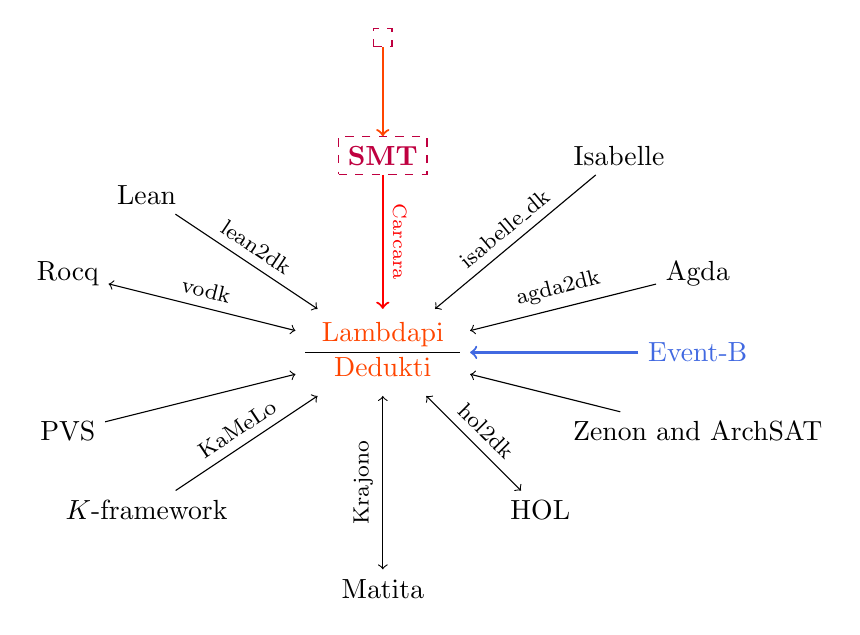
\begin{tikzpicture}
      \path (0,0) node (lp) {\begin{tabular}{c}
        \textcolor{OrangeRed}{Lambdapi} \\
        \hline
        \textcolor{OrangeRed}{Dedukti}
      \end{tabular}}
            (-4,1) node (coq) {Rocq}
            (-3,2) node (lean) {Lean}
            (0,2.5) node [draw, dashed, purple] (smt) {\color{purple}\textbf{SMT}}
            (0,4) node [draw, dashed, purple] (tla) {\color{purple}\tlaplus}
            (3,2.5) node (isa) {Isabelle}
            (4,1) node (agda) {Agda}
            (-3,-2) node (k) {$\mathbb{K}$-framework}
            (0,-3) node (mat) {Matita}
            (2,-2) node (hol) {HOL}
            (-4,-1) node (pvs) {PVS}
            (4,0) node (eventb) {\textcolor{RoyalBlue}{Event-B}}
            (4,-1) node (ze) {Zenon and ArchSAT}
            ;
      \draw[->,red, thick] (smt) -- (lp) node[midway,sloped,above]
      {\scriptsize{Carcara}};
      \draw[->,OrangeRed, thick] (tla) -- (smt) node[midway,sloped,above] {};
      \draw[->,RoyalBlue, thick] (eventb) -- (lp) node[midway,sloped,above] {};
      \draw[->] (lean) -- (lp) node[midway,sloped,above] {\footnotesize{lean2dk}};
      \draw[->] (isa) -- (lp) node[midway,sloped,above] {\footnotesize{isabelle\_dk}};
      \draw[->] (agda) -- (lp) node[midway,sloped,above] {\footnotesize{agda2dk}};
      \draw[->] (ze) -- (lp) node[midway,sloped,above] {};
      \draw[<->] (hol) -- (lp) node[midway,sloped,above] {\footnotesize{hol2dk}};
      \draw[<->] (mat) -- (lp) node[midway,sloped,above] {\footnotesize{Krajono}};
      \draw[->] (pvs) -- (lp);
      \draw[->] (k) -- (lp) node[midway,sloped,above] {\footnotesize{KaMeLo}};
      \draw[<->] (coq) -- (lp)  node[midway,sloped,above] {\footnotesize{vodk}};
    \end{tikzpicture}
    \caption{Verifying TLAPS proof with Lambdapi.}
    \label{fig:interop-tla}
\end{figure}

\paragraph{Sharing \tlaplus theorems}
The work presented in~\cite{eventb2lp} encodes the logic and set theory of Event-B in Lambdapi, enabling proof checking within a type-theoretical framework.
Event-B is a formal method for system-level modelling and verification, based on sorted set theory and first-order logic.
It shares key similarities with \tlaplus, particularly in its use of set-theoretical constructs, and its emphasis on proof obligations for correctness.
Given this proximity, as \cref{fig:interop-tla} suggests, a promising direction for future work would be to explore translations between \tlaplus and Event-B, possibly via a common intermediate representation in Lambdapi.
One possible approach to enable this transfer could build on the \emph{parametricity} \cite{theorem-for-free,parametricity} based methodology developed in \cite{parametricity-lp}, which provides a framework for connecting two theories encoded in Lambdapi. 
Such a translation path could allow one to leverage verification tools from both ecosystems while maintaining a shared logical foundation.

\paragraph{Lambdapi Hammer} This work lays the foundation for a future \emph{hammer} in Lambdapi similar to CoqHammer or Sledgehammer, to benefit from automatic proof reconstruction, assuming proper encoding of Lambdapi symbols in SMT.
A similar strategy to that employed by CoqHammer \cite{coqhammer1,coqhammer2}  could be pursued to realise this perspective.

\section{Summary}

In summary, this work establishes Lambdapi as a suitable backend for certifying SMT proofs and contributes a significant step towards making Alethe a widely usable standard for proof exchange in the formal methods community.
It opens the way for future extensions, in particular the support for additional theories such as bit-vectors and arrays, as well as tighter integration with interactive proof assistants.
Ultimately, the methodology proposed here strengthens the bridge between automated reasoning and interactive theorem proving, fostering greater confidence in the results of modern SMT solvers.
